\documentclass[../main.tex]{subfiles}

\begin{document}

\subsection{Governing Equation}

Consider the following radially symmetric cylindrical model. At a distance $x$ consider an infinitesimal slice of $dx$.

\begin{figure}[h]
    \centering
    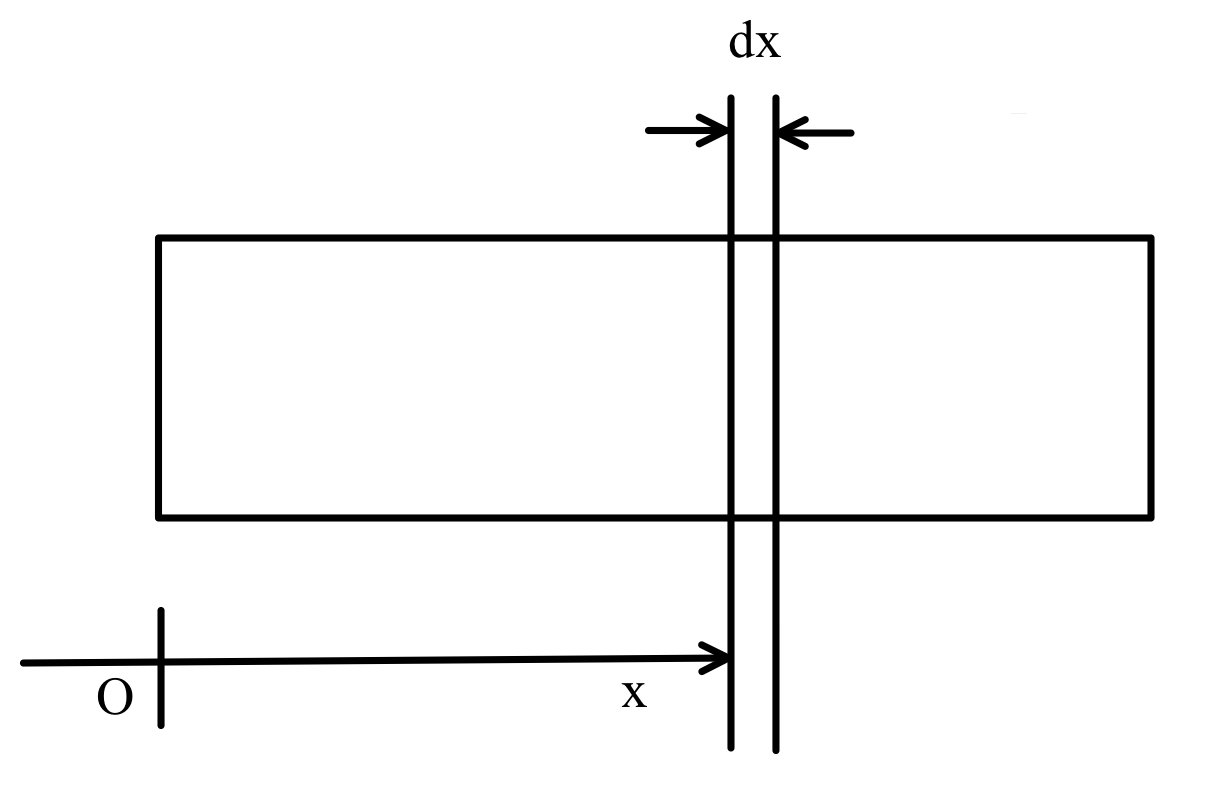
\includegraphics[scale=0.15]{images/schematic.png}
    \caption{Energy balance for an infinitesimal slice}
    \label{fig:my_label}
\end{figure}

\noindent The governing equation from energy balance for the infinitesimal slice is given by

\begin{equation}
    \rho_m C_{p,m} \frac{\partial T}{\partial t} =
    \lambda_m \frac{\partial^2 T}{\partial x^2}
    + \frac{\rho_m Q_r \dot{\omega}}{(MW)_{prod}}
    - \frac{4}{D} \left[ h \left( T - T_a \right) + \varepsilon \sigma \left( T^4 - T_a^4 \right) \right]
\end{equation}

\noindent The boundary conditions are

\begin{itemize}
    \item $T \left(t, x = 0 \right) = T_f$
    \item $\frac{\partial T}{\partial x} |_{t, x = L} = 0$
\end{itemize}

\noindent The initial condition is $T \left( t = 0, x \right) = T_u$

\subsection{Discretization}

\subsubsection{Temperature Predictor Step}

$$
\rho_m C_{p,m} \frac{\hat{T}_i - T^{n/k}_i}{\Delta t} =
\lambda_m \left\{ \frac{\hat{T}_{i+1} - 2\hat{T}_i + \hat{T}_{i-1}}{\left(\Delta x\right)^2} \right\}
$$

\begin{equation}
    \Rightarrow
    \left\{ \frac{\lambda_m}{\left(\Delta x\right)^2} \right\} \hat{T}_{i+1} -
    \left\{ 2\frac{\lambda_m}{\left(\Delta x\right)^2} + \frac{\rho_m C_{p,m}}{\Delta t} \right\} \hat{T}_i +
    \left\{ \frac{\lambda_m}{\left(\Delta x\right)^2} \right\} \hat{T}_{i-1} =
    - \left\{ \frac{\rho_m C_{p,m}}{\Delta t} \right\} T^{n/k}_i
\end{equation}

\subsubsection{Conversion Corrector Step}

\begin{equation}
    \eta^{n/k+1}_i = \frac{\eta^{n/k}_i + k \left(\hat{T}\right)\Delta t}{1 + k\left(\hat{T}\right)\Delta t}
\end{equation}

\subsubsection{Temperature Corrector Step}

$$
    \rho_m C_{p,m} \frac{T^{n/k+1}_i - \hat{T}_i}{\Delta t} = 
    \frac{\rho_m Q_r}{\left( MW \right)_{prod}} k\left( T^{n/k+1}_i \right) \left( 1 - \eta_i^{n/k+1} \right) -
    \frac{4h}{D} \left( T^{n/k+1}_i - T_a \right) -
    \frac{4 \varepsilon \sigma}{D} \left\{ \left( T^{n/k+1}_i \right)^4 - T_a^4 \right\}
$$
$$
    = \frac{\rho_m Q_r}{\left( MW \right)_{prod}} \left( 1 - \eta_i^{n/k+1} \right) \left\{ k\left(\hat{T}_i\right) + k'\left(\hat{T}_i\right)\left(T^{n/k+1}_i - \hat{T}_i\right) \right\}
$$
$$
    - \frac{4h}{D} \left( T^{n/k+1}_i - T_a \right)
    - \frac{4 \varepsilon \sigma}{D} \left\{ \hat{T}^4_i + 4\hat{T}^3_i\left( T^{n/k+1}_i - \hat{T}_i\right) - T_a^4 \right\}
$$

\begin{equation}
    T^{n/k+1}_i = 
    \frac{ \frac{\rho_m C_{p,m}}{\Delta t} \hat{T}_i +
    \frac{\rho_m Q_r}{\left( MW \right)_{prod}} \left( 1 - \eta_i^{n/k+1} \right) \left\{ k\left(\hat{T}_i\right) - k'\left(\hat{T}_i\right)\hat{T}_i \right\} +
    \frac{4h}{D} T_a +
    \frac{4 \varepsilon \sigma}{D} \left( 3\hat{T}^4_i + T_a^4 \right)}
    {\frac{\rho_m C_{p,m}}{\Delta t} +
    \frac{\rho_m Q_r}{\left( MW \right)_{prod}} \left( 1 - \eta_i^{n/k+1} \right) k'\left(\hat{T}_i\right) + 
    \frac{4h}{D} + 
    16 \frac{\varepsilon \sigma}{D} \hat{T}^3_i}
\end{equation}

\end{document}